\documentclass[]{report}

\usepackage[utf8]{inputenc}
\usepackage[T1]{fontenc}
\usepackage[francais]{babel}
\usepackage{graphicx}         % Pour les images
\usepackage{enumerate}
\usepackage{url}              % Pour les url et adresses e-mail

\begin{document}

\title{Title}
\author{Author}
\date{Today}
\maketitle

\tableofcontents

\chapter{Introduction}

\chapter{Présentation}
	\begin{itemize}
		\item{Nous + Tuteur}
	\end{itemize}
	
	\section{Projet}
		\begin{itemize}
			\item{On l'a proposé}
			\item{Principe du projet et description}
			\item{Rapprochement avec nos cours (I2A, Casar, Diwed)}
			\item{Buts / Attentes recherchés}
		\end{itemize}
		
	\section{Plate-formes de développement}
		\subsection{Android}
			\begin{itemize}
				\item{De qui ?}
				\item{Langage}
				\item{PC}
				\item{SDK - (le contenu)}
			\end{itemize}
		\subsection{iOS}
			\begin{itemize}
				\item{De qui ?}
				\item{Langage}
				\item{Mac}
				\item{SDK - (le contenu)}
			\end{itemize}
			
	\section{Organisation}
		\begin{itemize}
			\item{SVN}
			\item{Réunions}
			\item{Répartition du travail}
			\item{Diagramme de Gant}
		\end{itemize}
	
	
\chapter{Analyse}
	\begin{itemize}
		\item{Introduction}
	\end{itemize}
	
	\section{Cahier des charges}
		\subsection{Menus}
		
		Les menus se doivent d'être clairs et de rendre l'utilisation de
		l'application aisée. Il s'agit d'un jeu ne demandant aucune compétence
		particulière, il va donc toucher un public large et doit pouvoir convenir à
		tout utilisateur et cela passe d'abord par une navigation intuitive dans les
		menus.
		
		Nous avons pour ce faire établi un diagramme d'activité reflettant les
		différents parcours possibles par un utilisateur lors de sa navigation dans
		l'application.
		
		\subsection{Jeu}
		
		Le jeu est la partie la plus importante du projet. Il se decompose en trois parties : Le model, la vue et le controlleur. Le modèle est composé du moteur physique, du moteur de rendu ainsi que de la hierarchie de classe permettant de representer l'ensemble des objets du jeu. La vue quant à elle est composée d'objets graphiques simples (Bouttons, images, ... ) et d'une partie reprèsentant le jeu. Elle se doit d'être ergonomique et de permettre à l'utilisateur de pouvoir jouer très simplement. Le controlleur permettra de faire le lien entre les actions de l'utilisateur sur le modèle. Cette décomposition permettra dans le futur de pouvoir modifier facilement le modèle et/ou la vue.
		
		L'application se doit de pouvoir changer de langue, avec comme langues initiales le francais et l'anglais. Elle doit permettre à l'utilisateur de jouer à des parties solitaires ou multijoueurs. Ce dernier possèdera un compte hors ligne et en ligne.
		
		Le premier permetta de personnaliser son profil comme par exemple pour modifier la couleur du joueur ou encore changer son pseudo... Il servira aussi à enregistrer les informations et les preferences de connexion sur une base de donnée locale, mais aussi les scores du joueurs (nombre de parties gagnées ou perdus). Le jeu devra permettre à l'utilisateur de pouvoir créer différents comptes hors lignes en cas de partage de télephone avec un ami ou un membre de famille, pour pouvoir garder en mémoire ses scores et ses préferences.
		
		Le compte en ligne quand à lui servira seulement à établir une connexion avec le serveur distant pour pouvoir jouer en multijoueur.
		
		Un menu d'aide doit apparaitre pour pouvoir aider le joueur à comprendre le but du jeu et comment jouer. Ce dernier doit être simple et très explicite étant donné la large tranche d'age d'utilisateur que vise cette application.
		
		Ensuite un éditeur de carte permettra aux utilisateurs de créer un large choix de cartes, grâce à une multitude de différents objets qui composeront les cartes. Ces dernieres pourront être seulement utilisé en mode solitaire.
		
		Pour les parties solitaires une inteligence artificielle avec trois niveaux de difficulté devra permettre à un joueur debutant, intermédiaire ou confirmé de jouer comme bon lui semble pour pouvoir améliorer sa maniere de jouer.
		
		\subsection{Serveur}
		
		Ce serveur représente la partie réseau de notre projet. Il doit pouvoir
		rendre fonctionnel le jeux entre plusieurs téléphones (qu'ils soient de type
		iOS ou Android). Autrement dit il servira d'hebergeur pour les parties et
		il se chargera de faire s'interagir les joueurs, via leur mobile, entre eux.
		Nous parlons donc ici des parties multijoueurs.\\ 
		Il devra être capable d'enregistrer des inscriptions de nouveaux joueurs, avec
		 vérification qu'il n'y ait pas de doublons. Ces derniers seront inscrits dans la base de données du serveur. Les joueurs devraient ainsi
		pouvoir se connecter en utilisant le couple username / mot de passe. Suite à
		cela les utilisateurs seront à même de lister les parties en cours, ils
		pourront choisir de créer des parties ou de les rejoindres.\\
		Voilà concernant les fonctionnalités qui ont été demandé pour la partie
		serveur.
	
	\section{Modélisation}
		\subsection{Général}
			\begin{itemize}
				\item{Langage utilisé}
				\item{Tout en anglais}
				\item{Modèle Vue Contrôleur}
				\item{Documentation - (Javadoc / appledoc)}
			\end{itemize}
			
		\subsection{Menus}
		\begin{center}
			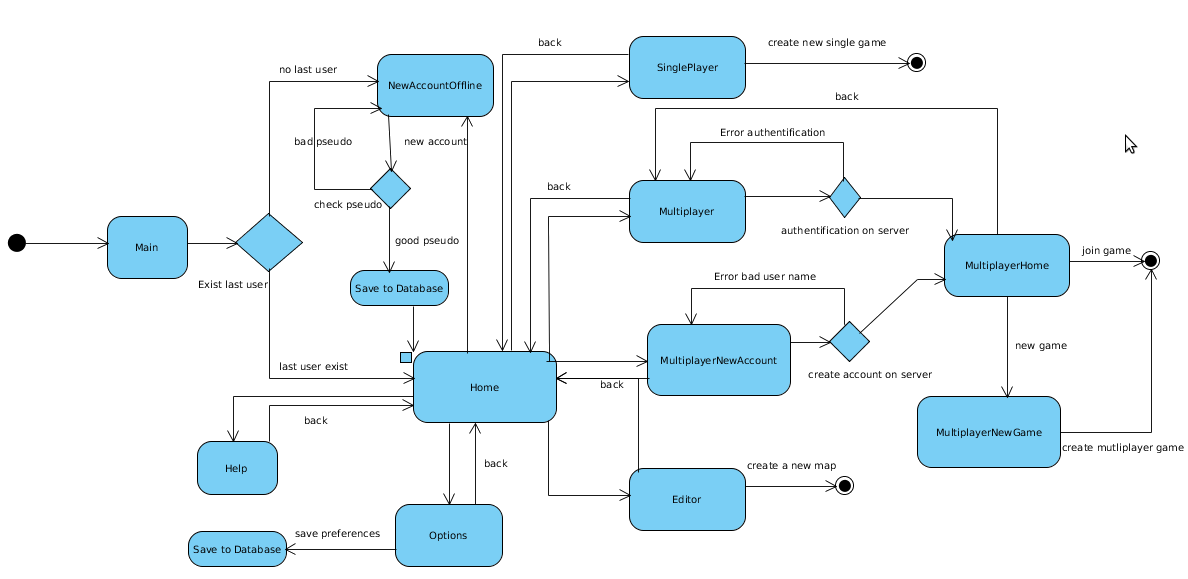
\includegraphics[width=16cm]{./ressources/diag_activity.png}
		\end{center}
		
			\begin{itemize}
				\item{Diagramme classe}
				\item{BDD (SQL-Lites)}\\
				
				
				\item{Scénarios}
				\item{utilisation des widgets des API}
			\end{itemize}
			
		\subsection{Jeu}
			\begin{itemize}
				\item{Diagramme classe}
				\item{Gameplay}
				\item{Gestion images / tile mapping}
				\item{Images}
				\item{Sons}
			\end{itemize}
			
		\subsection{Réseau}
			\begin{itemize}
				\item{J2EE --> Servlets}
				\item{Diagramme classe}
				\item{BDD (SQL-Lites)}
				\item{Protocoles du serveur (Json)}
			\end{itemize}
			
	\section{Différences entre Android et iOS}
	


\chapter{Développement}
	\section{Mobile}
		\subsection{Menus}
			\subsubsection{BDD}
			Après avoir effectués divers recherches, il s'est avéré que le gestionnaire
			de bases de données utilisé sur les deux plateformes est SQLite 3. 
			
			\paragraph{Android\\}
			
			Pour manipuler aisément les bases de données depuis l'application,
			nous avons crée une classe héritant de \textit{SQLiteOpenHelper}. Cette
			dernière fournit des outils de manipulations. Un attribut y est
			instancié, il s'agit de la base de données elle même, de type
			\textit{SQLiteDatabase}.
			
			Nous y avons crée 3 Tables, \textit{PlayerAccount} sauvegardant toutes les
			informations sur les utilisateurs locaux, \textit{System} concervant les
			propriétés du système, et enfin \textit{Map} décrivant les informations
			relatives au cartes de jeux crées par l'utilisateur.
			
			Ainsi de nombreuses	fonctions ont été implémenté dans le but de simplifier les interactions
			avec cette base de données depuis l'application. Il est par exemple possible de créer un nouvel 
			utilisateur local, modifier ses préférences, gérer les configurations systèmes comme la langue ou le volume
			du son, ajoûter de nouvelles maps ou même récupérer toutes les informations
			concernant un utilisateur.\\
			
			Voici un exemple d'insertion d'un nouveau compte local dans la base de
			donnée. Rappelons que les tests d'existance du compte ont été fait depuis
			l'application même. Dans cet exemple vous verrez ainsi que nous commençons
			par récupérer les droits en écritures sur la base de données locale, puis
			nous créons un container qui servira à l'insertion de valeur dans la base. Et
			enfin l'insertion est faite. Nous terminons tout de même en fermant l'accès à
			cette base.
			
			Il s'agit la d'un schéma classique de fonction d'interaction avec notre
			base.
						
			\begin{verbatim}
			/** ajout compte hors ligne **/
				public long newAccount(String nomCompte){
					base = getWritableDatabase();
			
					ContentValues entree = new ContentValues();
					
					entree.put("pseudo", nomCompte);
					long var = base.insert("PlayerAccount", null, entree);
					
					base.close();
					return var;
				}
			\end{verbatim}

			
			\paragraph{iOS}
				
			\subsubsection{Première utilisation}
			\subsubsection{Création utilisateur}
			\subsubsection{Gestion utilisateur}
			\subsubsection{Gestion des préférences système}
			\subsubsection{Création de carte (charger)}
			\subsubsection{Création partie solo (tout)}
			\subsubsection{Création partie multi (officielle)}
			
		\subsection{Editeur de carte}
			\subsubsection{Rendu}
			\subsubsection{Interface utilisateur}
			\subsubsection{Sauvegarde}
		\subsection{Jeu}
			\subsubsection{Moteurs}
				\paragraph{Rendu}
					\subparagraph{Structure utilisée}
					\begin{itemize}
						\item{Pourquoi}
						\item{Avantages}
					\end{itemize}
				\paragraph{Physique}
					\subparagraph{Structure utilisée}
					\subparagraph{Mouvements (collisions)}
					\subparagraph{Gestion des bombes}
						\begin{itemize}
							\item{Threads}
						\end{itemize}
			\subsubsection{IA}
				\paragraph{Pathfinding}
					\subparagraph{A*}
					\subparagraph{Aléatoire}
				\paragraph{Prise de décision}
			\subsubsection{Interface utilisaeur}
				\paragraph{Android}
				\paragraph{iOS}
		
	\section{Serveur}
		Nous avons choisi de créer notre serveur sur une base de servlet. Ce fût ici
		aussi un point nouveau pour nous, réiterant les phases d'analyse, de
		découverte, de test et de mise en place. Le fonctionnement est basé sur les
		échanges de requêtes type HTTP, où à chaque demande correspond une réponse. 
		
		\subsection{Json}
		Soucieux des performances et de la rapidité des échanges entre applications et
		serveur, nous avons mis en place un protocole de communication client/serveur
		où les messages transitant sont des flux JSON. Ce dernier semblait être un
		format de données d'échanges optimal pour véhiculer le plus d'informations
		avec une taille moindre. De plus étant beaucoup utilisé, nos deux langages
		mettent à disposition des outils de sérialisation de leurs objets en JSON.
		
		\begin{verbatim}
		ServletInscription
			Player => Serveur
			{["username","password"]}
			
			Serveur => Player
			{"OK"} ou {"BU"}
			
		ServletConnexion 	
			Player => Serveur
			{["username","password"]}
			
			Serveur => Player
			{"OK"} ou {"BU"}
			
		ServletGameList
			Player => Serveur
			{"userKey"}
		
			Serveur => Player
			{[{"class":"Game","map":"mapName","name":"gameName",
			 "playerNumberConnected":nbConnected,"type":"gameType"},{..},{..}]}
			 
		ServletCreateGame:
			Player => Server:
				{"userKey": <userKey>, "game": {"name":<name>, "type":<type>, "map":<map>, "ennemiesNumber": <ennemiesNumber>}}
				
			Server => Player:
				{"OK"} ou {"errorType"}
			 
		ServletConnectionGame:
			Player => Server:
				{["userKey", "gameName"]}
				
			Server => Player:
				{[<1/2/3/4>, "play<true/false>", "map", "time<mm:ss>"]} 
				ou 
				{"errorType"}
				
		ServletManageGame:
			Player => Server: 
				{"userKey", "gameName", "action"}	
				
			Server => Players: (Player, bombs, blocs, score, time)
				{[
				 [ ["x", "y", "direction", "dead <true/false>"],[...] ],
				 [ ["x", "y", "type", "explode <true/false>" ], [...] ],
				 [ ["position": {"x", "y"}, "bonus": <bonus>], [..] ],
				 [1,2,3,4],
				 "time <mm:ss>"]} 
				 ou 
				{"errorType"}
			 
			 
		\end{verbatim}
		
		\subsection{Servlet}
		Comme il a été dit précédement, notre serveur est accessible via des requêtes
		HTTP contactant des servlets. Ces servlets sont stockées dans un serveur
		d'application nommé Apache Tomcat. Il s'agit d'un conteneur libre de
		servlets Java 2 Enterprise Edition, mais il fait aussi office de serveur
		Web.
		
		Une servlet est une classe Java qui permet de créer dynamiquement des données
		au sein d'un serveur HTTP. Une servlet s'exécute dynamiquement sur le serveur
		web et permet l'extension des fonctions de ce dernier, typiquement : accès à
		des bases de données.
		
		\subsubsection{Schéma de fonctionnement }
		
		\begin{center}
			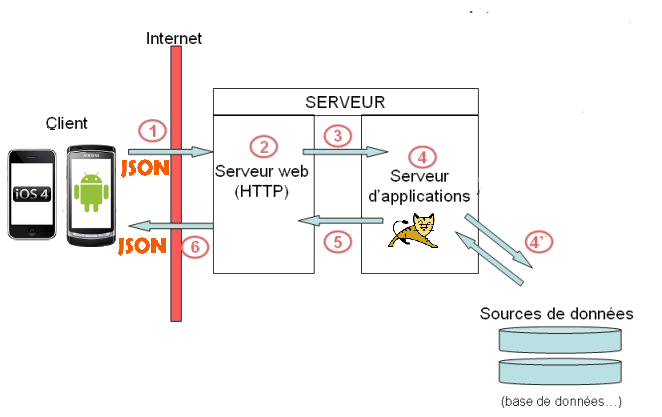
\includegraphics[width=16cm]{./ressources/serveurappli.png}
		\end{center}
		
		\begin{enumerate}[1]
		 \item Le client émet une requête pour demander une
			ressource au serveur. Par exemple la création de son compte multijoueur,
			qui pourrait se situer \url{http://Bomberklob.com/inscription}
		\item Côté serveur, c'est le serveur web qui traite les
			requêtes HTTP entrantes. Il traite donc toutes les requêtes, qu'elles
			demandent une ressource statique ou dynamique. Seulement, un serveur HTTP ne
			sait répondre qu'aux requêtes visant des ressources statiques.
		\item Ainsi, si le serveur HTTP s'aperçoit que la requête reçue est destinée
		au serveur d'applications, il la lui transmet. Les deux serveurs sont reliés par un canal, nommé connecteur.
		
		\item Le serveur d'applications (dans notre cas Tomcat) reçoit la requête à
		son tour. Lui est en mesure de la traiter. Il exécute donc la servlet
		correspondante à la requête, en fonction de l'URL, en récupérant les valeurs
		dans le flux JSON entrant. Cette opération est effectuée à partir de la
		configuration du serveur, grâce un fichier web.xml faisant le mapping entre URL et servlet associée. 
		
		La servlet est donc invoquée, et le serveur lui fournit notamment deux objets
		Java exploitables: un représentant la requête, l'autre représentant la réponse.
		La servlet execute sa fonction et génère la réponse à la demande, sous forme
		de flux JSON. Cela peut passer par la consultation de sources de données,
		comme des bases de données (4' sur le schéma).		
		
		\end{enumerate}
		
		
		\subsubsection{En pratique}
		
		Le requetes font appel la fonction post des servlet. Le flux entrant étant de
		type JSON, il faut déserialiser le flux dans un objet correspondant. Exemple
		l'utilisateur envoie son userName et son mot de passe crypté dans un tableau,
		sérialisé en JSON, pour pouvoir récupérer les informations nous procédons
		comme suit: 
		
		\begin{verbatim}
			BufferedReader req = 
				  new BufferedReader(new InputStreamReader(request.getInputStream()));
			OutputStreamWriter writer = 
				  new OutputStreamWriter(response.getOutputStream());
			String message = req.readLine();
			
			if (message != null) {
				  response.setContentType("text/html");
				
				   // désérialisation des infos de l'utilisateur dans une arraylist 
				  JSONDeserializer<ArrayList<String>> jsonDeserializer = 
					  new JSONDeserializer<ArrayList<String>>();
				  ArrayList<String> identifiers;
				  identifiers = jsonDeserializer.deserialize(message);
				
				  username = identifiers.get(0);
				  password = identifiers.get(1);
				  
			  ...}
		\end{verbatim}
		
		
		\subsubsection{La sécurité}
		S'agissant d'un jeux ouvert sur internet avec 
		
		
		\subsection{BDD}
		
		
\chapter{Manuel d'utilisation}
	\section{Menus}
	\section{Jeu}
	\section{Editeur}
	

\chapter{Discussion}
	\section{Problèmes}
		\subsection{Android}
		\subsection{iOS}
	\section{Améliorations}
		\subsection{Jeu}
		\subsection{Serveur}
			\begin{itemize}
				\item{Pooling}
				\item{Session}
			\end{itemize}
			
\chapter{Conclusion}

\end{document}
